In dit deel zullen de resultaten van de testen toegelicht worden, deze zijn onderverdeeld in: de grafische testen, de Physics test en de algemene scores berekend volgens de formules vermeld in sectie 3.

\subsection{Grafische testen}

Deze test legt de nadruk eerder op de grafische processor van de laptop, als we de laptops bekijken dan mogen we vrij zeker zijn dat de MSI GT72 er bovenuit zal steken door zijn nieuwere en sterke grafische kaart. Hier is de bijhorende grafiek: \\
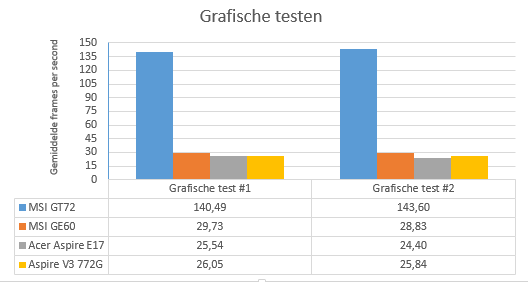
\includegraphics[width=8cm]{grafische}\\
Zoals verwacht steekt de GT72 hier met kop en schouders bovenuit door zijn grafische kaart (GTX980M) deze is voor het moment de nieuwste versie voor de NVIDIA chipset.\\
De GE60 & de Aspire V3 772G dezelfde grafische kaart hebben is er een klein verschil in performantie, de GE60 zijn performantie ligt iets hoger.
Het vreemde is dat de Aspire E17 een nieuwere grafische kaart heeft maar toch een gelijkaardige performantie heeft aan de andere twee, dit komt door dat de GPU's die eindigen met 50 en hoger mid tot high-end zijn maar die eronder worden verondersteld van low-end te zijn.

\subsection{Physics test}

Zoals vermeld in sectie 3 is deze test meer op de Processor gericht, als we naar de tabel kijken zien we dat de GT72 de nieuwste generatie CPU heeft, de GE60 en de Aspire V3 hebben dezelfde generatie CPU en de Aspire E17 heeft een iets zwakkere CPU.\\
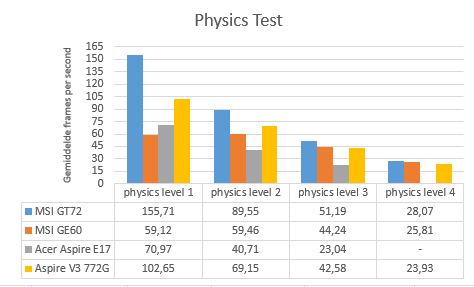
\includegraphics[width=8cm]{physics}\\
Deze test wordt opgedeeld in vier testen zoals vermeld in sectie 3.2.2, we zien dat de GT72 in het eerste level een veel hogere performantie heeft dan de rest, verassend zien we ook dat de GE60 een aanzienlijk lagere score heeft als het om weinig objecten tegelijk draait.
Wanneer we het tweede level bekijken zien we dat de performantie van de Aspire E17 heel hard is afgevallen en dat de GE60 en Aspire V3 min of meer gelijkgekomen zijn maar de Aspire V3 steekt er nog steeds iets boven.
Bij het derde niveau is de GT72 zijn performantie sterk aan het gelijkkomen met die van de GE60 en de Aspire V3 terwijl de Aspire E17 verder afvalt.
Bij het laatste niveau kunnen we concluderen dat deze CPU's weinig onderscheid hebben als het draait om zoveel berekeningen tegelijk. Er is geen resultaat bij level 4 bij de Aspire E17 omdat het aantal frames per seconde dat de laptop haalt onder de minimum threshold valt voor deze test. Dit zou betekenen dat het ongezond zou zijn voor de processor om deze test te vervolledigen.

\subsection{Scores}
